\section{Case Studies}

In addition to the somewhat artificial Simplified Arbiter,
we tested our technique on two representative problems:
\begin{paragraph}{Gap problem.}
A generalized minimal edit distance problem. Given two input strings 
$\overline{x}=x_1\cdots x_m$ and $\overline{y}=y_1\cdots y_n$,
compute the cost of transforming $x$ into $y$ by any combination of the
following steps
\begin{itemize}
  \item Replacing $x_i$ with $y_j$, at cost $c_{ij}$.
  \item Deleting $x_{p+1}\cdots x_q$, at cost $w_{pq}$.
  \item Inserting $y_{p+1}\cdots y_q$ in $\overline{x}$, at cost $w'_{pq}$.
\end{itemize}

The computation is given by the recurrence \Cref{evaluation:gap spec}.
\end{paragraph}

\begin{paragraph}{Parenthesis problem.} Compute
an optimal placements of parenthesis in a long chain of multiplication, e.g. of matrices, where the input is
are cost functions $x_i$ for accessing the $i$-th element and
$w_{ikj}$ for multiplying elements $[i,k)$ by elements $[k,j)$.
The corresponding recurrence is shown in \Cref{evaluation:paren spec}.
\end{paragraph}

\begin{figure}
\[
  \renewcommand\arraystretch{1.5}
  \begin{array}{@{}l@{}l@{}l@{}}
    \lspan3{w :: ((J\times J)\cap{<})\to\R} \\
    \lspan3{w' :: ((K\times K)\cap{<})\to\R} \\
    G ~=~ \fix \theta\,i\,j\mapsto{}
      & \lspan2{0\big|_{i=0\land j=0} ~\Big/~ w'_{0j}\big|_{i=0} ~\Big/~ w_{i0}\big|_{j=0} ~\Big/~} \\
      & \min~\langle~ & \theta_{(i-1)\,(j-1)} + c_{ij},\\
      & & \min p\mapsto\theta_{pj}+w_{pi}, \\
      & & \min q\mapsto\theta_{iq}+w'_{qj} ~\rangle
  \end{array}
\]
\caption{\label{evaluation:gap spec}
  Specifications for the full version of the Gap DP problem.}
\end{figure}

\begin{figure}
\[
  \renewcommand\arraystretch{1.5}
  \begin{array}{@{}l@{}l}
    \lspan2{x :: J\to\R} \\
    \lspan2{w :: (J\times J\times J)\to\R} \\
    E ~=~ \fix \theta\,i\,j\mapsto{}
      & {x_{ij}\big|_{i+1=j} ~\Big/~} \\
      & \min k\mapsto\theta_{ik}+\theta_{kj}+w_{ikj} \\
  \end{array}
\]
\caption{\label{evaluation:paren spec}
  Specifications for the Parenthesis Assignment DP problem.}
\end{figure}


The next example shows more steps for the Simplified Arbiter test case.

\exampleTitle
\begin{comment}\subsection{Example}\end{comment}

Further developing $A^{IJ}$ \eqref{tactics:arbiter phase A}
we apply Slice to get the four quadrants; $I_0$, $I_1$, $J_0$, $J_1$
(\Cref{intro:quadrants}) are defined as unary qualifiers with the axioms:
\[
\begin{array}{c@{\qquad}c}
  \forall i{:}I.~~I_0(i)\lor I_1(i)   &    \forall i_0{:}I_0,~i_1{:}I_1.~~i_0<i_1 \\
  \forall j{:}J.~~J_0(j)\lor J_1(j)   &    \forall j_0{:}J_0,~j_1{:}J_1.~~j_0<j_1 \\
\end{array}
\]

As a result, the term is
going to grow quite large; to make such terms easy to read and refer to, we provide
boxed letters as labels for sub-terms, using them as abbreviations where they
occur in the larger expression.

\makeatletter
\newcommand{\quadrants@normal}[4]{
  \renewcommand\arraystretch{1.5}
   \begin{array}{c|c}
     #1 & #2 \\ \hline
     #3 & #4
   \end{array}}
\newcommand{\quadrants@small}[4]{
  \renewcommand\arraystretch{0.9}
   \begin{array}{@{~}c@{~}|@{~}c@{~}}
     \scriptstyle #1 & \scriptstyle #2 \\ \hline
     \scriptstyle #3 & \scriptstyle #4
   \end{array}}
\newcommand\quadrants{\@ifstar\quadrants@small\quadrants@normal}
\makeatother

In addition, to allude to the reader's intuition, expressions of the form
$a/b/c/d$ will be written as $\quadrants*{a}{b}{c}{d}$ when the slices
represent quadrants.

\makeatletter
\newcommand{\lbox@small}[1]{ {\setlength{\fboxsep}{1pt}\fbox{\small #1}} }
\newcommand{\lbox@tiny}[1]{ {\setlength{\fboxsep}{1pt}\fbox{\tiny #1}} }
\newcommand\lbox{\@ifstar\lbox@tiny\lbox@small}
\makeatother

\begin{center}
\fbox{$\begin{array}{ll}
       \mbox{\underline{Slice}} \\ 
       f ~=~ \theta\,i\,j\mapsto \cdots \\
       X_1 ~=~ \_\times I_0\times J_0 &
       X_2 ~=~ \_\times I_0\times J_1 \\
       X_3 ~=~ \_\times I_1\times J_0 &
       X_4 ~=~ \_\times I_1\times J_1 \\[.5em]
       \cspan2{\mbox{\small ({\it recall that each} ``\_'' {\it is a fresh type variable})}}
       \end{array}$}
\end{center}

\begin{equation}
  \renewcommand\arraystretch{1.2}
  \begin{array}{@{}r@{}l@{}c@{}c@{}l@{}l@{}}
    A^{^{IJ}} =~ & \lspan5{\psi\mapsto \fix \quadrants{\lbox A}{\lbox B}{\lbox C}{\lbox D}} \\
	\lbox A ~=~ & \theta\,& i & j & \mapsto\min\,\langle~ & \psi_{ij} \\
	      & & ^{^{(I_0)}} & ^{^{(J_0)}} & & \min \vtyped p I \mapsto\theta_{pj}+w_{pij}, \\
	      & & & & & \min \vtyped q J \mapsto\theta_{iq}+w'_{qji} ~\rangle \\
	\lbox B ~=~ & \theta\,& i & j & \mapsto\min\,\langle~ & \psi_{ij} \\
	      & & ^{^{(I_0)}} & ^{^{(J_1)}} & & \min \vtyped p I \mapsto\theta_{pj}+w_{pij}, \\
	      & & & & & \min \vtyped q J \mapsto\theta_{iq}+w'_{qji} ~\rangle \\
	\lbox C ~=~ & \theta\,& i & j & \mapsto\min\,\langle~ & \psi_{ij} \\
	      & & ^{^{(I_1)}} & ^{^{(J_0)}} & & \min \vtyped p I \mapsto\theta_{pj}+w_{pij}, \\
	      & & & & & \min \vtyped q J \mapsto\theta_{iq}+w'_{qji} ~\rangle \\
	\lbox D ~=~ & \theta\,& i & j & \mapsto\min\,\langle~ & \psi_{ij} \\
	      & & ^{^{(I_1)}} & ^{^{(J_1)}} & & \min \vtyped p I \mapsto\theta_{pj}+w_{pij}, \\
	      & & & & & \min \vtyped q J \mapsto\theta_{iq}+w'_{qji} ~\rangle \\
  \end{array}
  \label{tactics:A sliced}
\end{equation}

\begin{tacticbox}{Let}
   e[\square] ~=~ \quadrants*{\square}{\lbox*B}{\lbox*C}{\lbox*D} \qquad
   t ~=~ \lbox A
\end{tacticbox}

\begin{equation}
  A^{^{IJ}} =~ \psi\mapsto \fix \left(\lbox A \applt z\mapsto\quadrants{z}{\lbox B}{\lbox C}{\lbox D}\right)
\end{equation}

\begin{tacticbox}{Stratify[with Padding]}
  \begin{array}{@{} l @{} l @{}}
    f ~=~ \quadrants*{\lbox*A}{\dot\psi}{\dot\psi}{\dot\psi}
         & \mbox{\small ({\it recall that } $\dot\psi=\theta\mapsto\psi$)} \\
    g ~=~ z\mapsto\quadrants*{z}{\lbox*{B}}{\lbox*C}{\lbox*D} &
    \qquad\psi=\psi
  \end{array}
\end{tacticbox}

\begin{equation}
  A^{^{IJ}} =~ \psi\mapsto \fix \quadrants{\lbox A}{\dot\psi}{\dot\psi}{\dot\psi} ~\applt~ \psi\mapsto\fix\quadrants{\dot\psi}{\lbox B}{\lbox C}{\lbox D}
\end{equation}

Notice that an existing variable $\psi$ is reused, rebinding any occurrences within $\lbox B$, $\lbox C$, $\lbox D$.
This effect is useful, as it limits the context of the expression: the inner $\psi$ shadows the outer $\psi$,
meaning $\lbox B$, $\lbox C$, $\lbox D$ do not need to access the data that was input to $\lbox A$, only its
output.

\medskip
The sequence Let, Stratify[with Padding] is now applied in the same manner to $\lbox B$
and $\lbox C$ (see \Cref{evaluation:stratify A}). We do not list the applications as they are analogous to the previous ones.

\begin{equation}
  \renewcommand\arraystretch{1.5}
  \begin{array}{l@{}l}
    A^{^{IJ}} =~ \psi\mapsto{} & \fix \quadrants{\lbox A}{\dot\psi}{\dot\psi}{\dot\psi} ~\applt~ 
                 \psi\mapsto\fix\quadrants{\dot\psi}{\lbox B}{\dot\psi}{\dot\psi} ~\applt \\
               & \psi\mapsto\fix\quadrants{\dot\psi}{\dot\psi}{\lbox C}{\dot\psi} ~\applt~
                 \psi\mapsto\fix\quadrants{\dot\psi}{\dot\psi}{\dot\psi}{\lbox D}
  \end{array}
\end{equation}

\begin{figure}
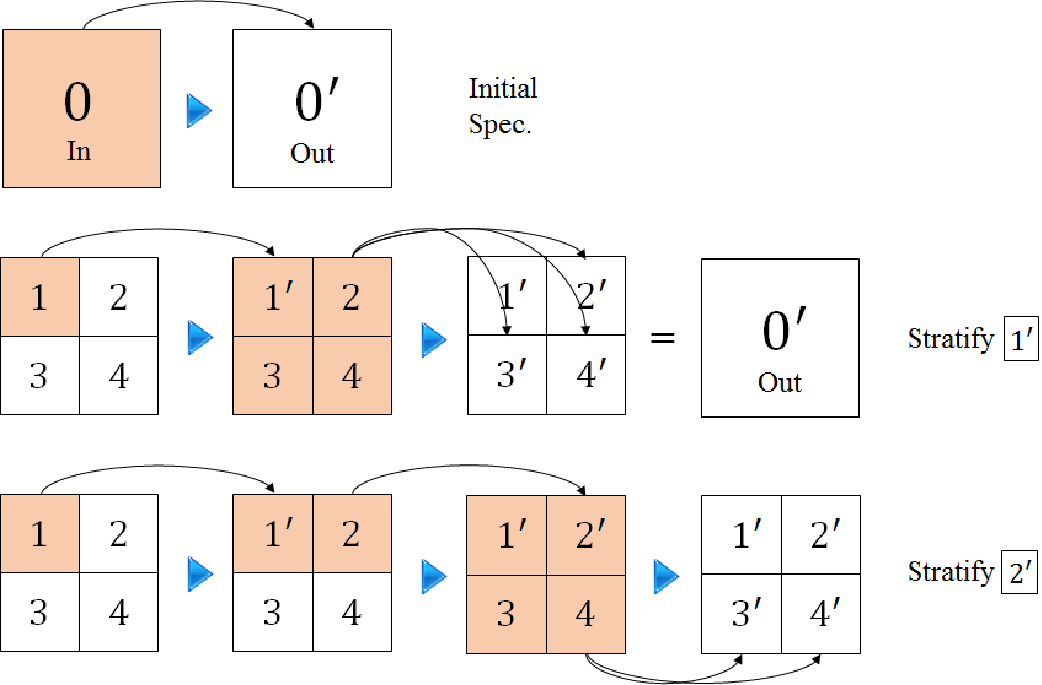
\includegraphics[width=.47\textwidth]{img/arbiter-stratify2}\\
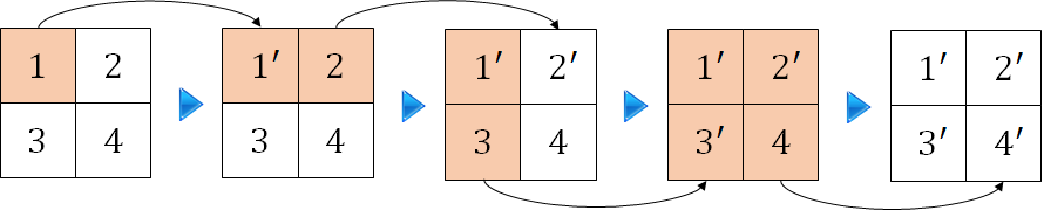
\includegraphics[width=.47\textwidth]{img/arbiter-stratify3}
\caption{\label{evaluation:stratify A}
  Stratification steps for phase ``A'' of Simplified Arbiter.}
\end{figure}

\begin{tacticbox}{Synth}
	\begin{array}{@{}l@{}c@{}c@{}l@{}l}
       \lspan5{h_1= \lbox A} \\
       \lspan5{h_{2,3,4}=\dot\psi} \\
	   f_1 = \theta\,& i & j & \mapsto\min\,\langle~ & \psi_{ij} \\
	      & ^{^{(I_0)}} & ^{^{(J_0)}} & & \min \vtyped p {I_0} \mapsto\theta_{pj}+w_{pij}, \\
	      & & & & \min \vtyped q {J_0} \mapsto\theta_{iq}+w'_{qji} ~\rangle \\
	   \lspan5{f_{2,3,4} = \dot\psi}
   \end{array}
\end{tacticbox}

\begin{equation}
  \renewcommand\arraystretch{1.5}
  \begin{array}{l@{}l}
    A^{^{IJ}} =~ \psi\mapsto{} & \quadrants{A^{^{I_0J_0}}_\psi\!\!\!}{\psi}{\psi}{\psi} ~\applt~ 
                 \psi\mapsto\fix\quadrants{\dot\psi}{\lbox B}{\dot\psi}{\dot\psi} ~\applt \\
               & \psi\mapsto\fix\quadrants{\dot\psi}{\dot\psi}{\lbox C}{\dot\psi} ~\applt~
                 \psi\mapsto\fix\quadrants{\dot\psi}{\dot\psi}{\dot\psi}{\lbox D}
  \end{array}
  \label{fix A}
\end{equation}

We note that $\fix f_1=A^{^{I_0J_0}}_\psi$ are identical up to $\beta$-reduction. Also, we took the liberty
to simplify $\fix\dot\psi$ into $\psi$ --- although this is not necessary --- just to display
a shorter term.

\medskip
The next few tactics will focus on the subterm $\lbox B$ from \eqref{tactics:A sliced}.

\begin{equation}
  \renewcommand\arraystretch{1.2}
  \begin{array}{@{}r@{}l@{}c@{}c@{}l@{}l@{}}
	\lbox B ~=~ & \theta\,& i & j & \mapsto\min\,\langle~ & \psi_{ij} \\
	      & & ^{^{(I_0)}} & ^{^{(J_1)}} & & \min \vtyped p I \mapsto\theta_{pj}+w_{pij}, \\
	      & & & & & \min \vtyped q J \mapsto\theta_{iq}+w'_{qji} ~\rangle
  \end{array}
\end{equation}

\begin{tacticbox}{Slice}
  \begin{array}{@{} l @{}}
    f = \vtyped q J \mapsto \theta_{iq}+w'_{qji} \\
    X_1 = J_0\to\_ \qquad X_2 = J_1\to\_
  \end{array}
\end{tacticbox}

\begin{equation}
  \renewcommand\arraystretch{1.2}
  \begin{array}{@{}r@{}l@{}c@{}c@{}l@{}l@{}l@{}}
	\lbox B ~=~ & \theta\,& i & j & \mapsto\min\,\big\langle~ & \psi_{ij} \\
	      & & ^{^{(I_0)}} & ^{^{(J_1)}} & & \lspan2{\min \vtyped p I \mapsto\theta_{pj}+w_{pij},} \\
	      & & & & & \min \big( & (\vtyped q {J_0} \mapsto\theta_{iq}+w'_{qji}) ~\big/~ \\
	      & & & & & & (\vtyped q {J_1} \mapsto\theta_{iq}+w'_{qji})\big)  ~\big\rangle
  \end{array}
  \label{evaluation:horiz sliced}
\end{equation}

For the intuition behind this, see the top-right part of \Cref{evaluation:slicing strategy}.
The colors represent cell ranges that will be read by different sub-routines (presumably running on different cores).
The range of $q$ is split into the part that lies within \qbox1 ($q\in J_0$) and the one that
lies within \lbox2 ($q\in J_1$). The same reasoning is applied to the other quadrants.

\begin{tacticbox}{Distributivity}
  \begin{array}{@{} l @{}}
    e[\square] = \min\square \\
    t_1 = \min \vtyped q {J_0} \mapsto \theta_{iq}+w'_{qji} \\
    t_2 = \min \vtyped q {J_1} \mapsto \theta_{iq}+w'_{qji} \\
  \end{array}
\end{tacticbox}

\begin{tacticbox}{Associativity}
  \begin{array}{@{} l @{} l @{}}
    \lspan2{\reduce = \min} \\
    \overline x_1 ={} & \psi_{ij} \\
    \overline x_2 ={} & \min \vtyped p I \mapsto\theta_{pj}+w_{pij} \\
    \overline x_3 ={} & \min \vtyped q {J_0} \mapsto \theta_{iq}+w'_{qji} ~, \\
                      & \min \vtyped q {J_1} \mapsto \theta_{iq}+w'_{qji}
  \end{array}
\end{tacticbox}

\begin{equation}
  \renewcommand\arraystretch{1.2}
  \begin{array}{@{}r@{}l@{}c@{}c@{}l@{}l@{}}
	\lbox B ~=~ & \theta\,& i & j & \mapsto\min\,\big\langle~ & \psi_{ij} \\
	      & & ^{^{(I_0)}} & ^{^{(J_1)}} & & \min \vtyped p I \mapsto\theta_{pj}+w_{pij}, \\
	      & & & & & \min \vtyped q {J_0} \mapsto\theta_{iq}+w'_{qji}, \\
	      & & & & & \min \vtyped q {J_1} \mapsto\theta_{iq}+w'_{qji} ~\big\rangle
  \end{array}
\end{equation}

\begin{tacticbox}{Let[$\reduce$]}
  \begin{array}{@{} r @{} l @{}}
    e[\square] ={} & \quadrants{\dot\psi}{\theta\,i\,j\mapsto\square}{\dot\psi}{\dot\psi} \\
    \overline a ={} & \psi_{ij}, ~\min \vtyped q{J_0}\mapsto \theta_{iq}+w'_{qji} \\
    \overline b ={} & \min \vtyped p I \mapsto\theta_{pj}+w_{pij}, \\
                    & \min \vtyped q {J_1} \mapsto\theta_{iq}+w'_{qji}
  \end{array}
\end{tacticbox}

\begin{equation}
  \renewcommand\arraystretch{1.2}
  \begin{array}{r @{} l @{} c @{} c @{} l @{} l}
    \lspan6{
    \quadrants{\dot\psi}{\lbox B}{\dot\psi}{\dot\psi} =
      \fix\left(\lbox E \applt z\mapsto\quadrants{\dot\psi}{\lbox F}{\dot\psi}{\dot\psi}\right) 
    } \\[1.5em]
    ~\lbox E ={} &
      \theta & i & j & \mapsto\min\langle & \psi_{ij}, \\
             & & ^{^{(I_0)}} & ^{^{(J_1)}} &
                                          & \min \vtyped q{J_0}\mapsto\theta_{iq}+w'_{qji} \rangle \\
    ~\lbox F ={} &
      \theta & i & j & \mapsto\min\langle & z_{\theta ij}, \\
             & & ^{^{(I_0)}} & ^{^{(J_1)}} &
                                         & \min \vtyped p I \mapsto\theta_{pj}+w_{pij}, \\
             & & & &                     & \min \vtyped q {J_1} \mapsto\theta_{iq}+w'_{qji}\rangle
  \end{array}
\end{equation}


\begin{figure}
\begin{tikzpicture}[x=4mm,y=4mm, node distance=1cm,
    slicer/.style={ultra thick},
    cell/.style={thick}, dot/.style={fill=BrickRed},
    block C/.style={fill=OliveGreen, fill opacity=0.2},
    block B/.style={fill=Orange, fill opacity=0.2},
    block A/.style={fill=Purple, fill opacity=0.2},
    label position=right,label distance=1pt,every label/.style={inner sep=0}]
  \draw[help lines] (0,0) grid[step=1] (8,8);
  \draw[slicer] (4,0) -- (4,8) (0,4) -- (8,4);
  \fill[block A] (0,5) rectangle (2,6) rectangle (3,8);
  \draw[cell] (2,5) rectangle +(1,1); \path[dot] (2.5,5.5) circle (1.5pt);
  \path (2,8) node[above] {$q\in J_0$} (6,8) node[above] {$q\in J_1$};
  \path (0,0) -- node[midway,above,sloped] {$p\in I_1$} (0,4)
              -- node[midway,above,sloped] {$p\in I_0$} (0,8);

  \tikzset{xshift=4cm}

  \draw[help lines] (0,0) grid[step=1] (8,8);
  \draw[slicer] (4,0) -- +(0,8) (0,4) -- +(8,0);
  \fill[block B] (0,5) rectangle (4,6);
  \fill[block A] (4,5) rectangle (6,6) rectangle (7,8);
  \draw[cell] (6,5) rectangle +(1,1); \path[dot] (6.5,5.5) circle (1.5pt);
  \path (2,8) node[above] {$q\in J_0$} (6,8) node[above] {$q\in J_1$};
  \path (0,0) -- node[midway,above,sloped] {$p\in I_1$} (0,4)
              -- node[midway,above,sloped] {$p\in I_0$} (0,8);
              
  \tikzset{yshift=-4cm,xshift=-4cm}
  
  \draw[help lines] (0,0) grid[step=1] (8,8);
  \draw[slicer] (4,0) -- +(0,8) (0,4) -- +(8,0);
  \fill[block C] (2,4) rectangle (3,8);
  \fill[block A] (0,1) rectangle (2,2) rectangle (3,4);
  \draw[cell] (2,1) rectangle +(1,1); \path[dot] (2.5,1.5) circle (1.5pt);
  \path (2,8) node[above] {$q\in J_0$} (6,8) node[above] {$q\in J_1$};
  \path (0,0) -- node[midway,above,sloped] {$p\in I_1$} (0,4)
              -- node[midway,above,sloped] {$p\in I_0$} (0,8);

  \tikzset{xshift=4cm}
  
  \draw[help lines] (0,0) grid[step=1] (8,8);
  \draw[slicer] (4,0) -- +(0,8) (0,4) -- +(8,0);
  \fill[block C] (6,4) rectangle (7,8);
  \fill[block B] (0,1) rectangle (4,2);
  \fill[block A] (4,1) rectangle (6,2) rectangle (7,4);
  \draw[cell] (6,1) rectangle +(1,1); \path[dot] (6.5,1.5) circle (1.5pt);
  \path (2,8) node[above] {$q\in J_0$} (6,8) node[above] {$q\in J_1$};
  \path (0,0) -- node[midway,above,sloped] {$p\in I_1$} (0,4)
              -- node[midway,above,sloped] {$p\in I_0$} (0,8);
  
  \tikzset{yshift=-.7cm,xshift=-2cm}
  
  \node(A)[rectangle,label=$A$,block A] {};
  \node(B)[right=of A,rectangle,label=$B$,block B] {};
  \node(C)[right=of B,rectangle,label=$C$,block C] {};
  
\end{tikzpicture}
\medskip
\caption{\label{evaluation:slicing strategy}
  The strategy for applications of Slice in the case study.}
\end{figure}

\begin{tacticbox}{Stratify[with Padding]}
  \begin{array}{@{} l @{}}
    f ~=~ \quadrants*{\dot\psi}{\lbox*E}{\dot\psi}{\dot\psi} \\
    g ~=~ z\mapsto\quadrants*{\dot\psi}{\lbox*F}{\dot\psi}{\dot\psi}
    \qquad\psi=\psi
  \end{array}
\end{tacticbox}

\begin{equation}
  \renewcommand\arraystretch{1.2}
  \begin{array}{r @{} l @{} c @{} c @{} l @{} l}
    \lspan6{
    \fix\quadrants{\dot\psi}{\lbox B}{\dot\psi}{\dot\psi} =
      \fix\quadrants{\dot\psi}{\lbox E}{\dot\psi}{\dot\psi} \applt
      \psi\mapsto\fix\quadrants{\dot\psi}{\lbox F}{\dot\psi}{\dot\psi}
    } \\[1.5em]
    ~\lbox E ={} &
      \theta & i & j & \mapsto\min\langle & \psi_{ij}, \\
             & & ^{^{(I_0)}} & ^{^{(J_1)}} &
                                          & \min \vtyped q{J_0}\mapsto\theta_{iq}+w'_{qji} \rangle \\
    ~\lbox F ={} &
      \theta & i & j & \mapsto\min\langle & \psi_{ij}, \\
             & & ^{^{(I_0)}} & ^{^{(J_1)}} &
                                          & \min \vtyped p I \mapsto\theta_{pj}+w_{pij}, \\
             & & & &                      & \min \vtyped q {J_1} \mapsto\theta_{iq}+w'_{qji}\rangle
  \end{array}
\end{equation}

\noindent
Define
\begin{equation}
  \renewcommand\arraystretch{1.2}
  \begin{array}{@{}l @{} l @{\!} c @{} c @{} l @{} l@{}}
  B^{^{IJ_0J_1}} =~ \big( & \psi\mapsto \\
      & \fix
      \theta & i & j & \mapsto\min\langle & \psi_{ij}, \\
           & & ^{^{(I)}} & ^{^{(J)}} &
                                          & \min \vtyped q{J_0}\mapsto\theta_{iq}+w'_{qji} \rangle\big) \\
      & \lspan5{:: \big((I\times J_0)\to\R\big) \to \big((I\times J_1)\to\R\big)}
  \end{array}
\end{equation}

\begin{tacticbox}{Synth}
  \begin{array}{@{} l @{} c @{} c @{} l @{} l @{}}
    \lspan5{h_2 = \lbox E} \\
    \lspan5{h_{1,3,4} = \dot\psi} \\
    f_2 = 
      \theta & i & j & \mapsto\min\langle & \psi_{ij}, \\
             & ^{^{(I_0)}} & ^{^{(J_1)}} &
                                          & \min \vtyped q {J_0} \mapsto\theta_{iq}+w'_{qji}\rangle \\
    \lspan5{f_{1,3,4} = \dot\psi}
  \end{array}
\end{tacticbox}

\begin{tacticbox}{Synth}
  \begin{array}{@{} l @{} c @{} c @{} l @{} l @{}}
    \lspan5{h_2 = \lbox F} \\
    \lspan5{h_{1,3,4} = \dot\psi} \\
    f_2 = 
      \theta & i & j & \mapsto\min\langle & \psi_{ij}, \\
             & ^{^{(I_0)}} & ^{^{(J_1)}} &
                                          & \min \vtyped p {I_0} \mapsto\theta_{pj}+w_{pij}, \\
             & & &                        & \min \vtyped q {J_1} \mapsto\theta_{iq}+w'_{qji}\rangle \\
    \lspan5{f_{1,3,4} = \dot\psi}
  \end{array}
\end{tacticbox}

\begin{equation}
  \fix\quadrants{\dot\psi}{\lbox B}{\dot\psi}{\dot\psi} ~=~
    \quadrants{\psi}{B^{^{I_0J_0J_1}}_\psi\!\!\!\!}{\psi}{\psi} ~\applt~
    \psi\mapsto\quadrants{\psi}{A^{^{I_0J_1}}_\psi\!\!\!}{\psi}{\psi}
  \label{fix B}
\end{equation}

\medskip\noindent
In a similar manner, we will obtain the following:

\begin{equation}
  \fix\quadrants{\dot\psi}{\dot\psi}{\lbox C}{\dot\psi} ~=~
    \quadrants{\psi}{\psi}{C^{^{I_0I_1J_0}}_\psi\!\!\!\!}{\psi} ~\applt~
    \psi\mapsto\quadrants{\psi}{\psi}{A^{^{I_1J_0}}_\psi\!\!\!}{\psi}
  \label{fix C}
\end{equation}

\begin{equation}
  \renewcommand\arraystretch{1.2}
  \begin{array}{@{}l @{} l @{\!} c @{} c @{} l @{} l@{}}
  C^{^{I_0I_1J}} =~ \big( & \psi\mapsto \\
      & \fix
      \theta & i & j & \mapsto\min\langle & \psi_{ij}, \\
           & & ^{^{(I)}} & ^{^{(J)}} &
                                          & \min \vtyped p {I_0} \mapsto\theta_{pj}+w_{pij} \rangle\big) \\
      & \lspan5{:: \big((I_0\times J)\to\R\big) \to \big((I_1\times J)\to\R\big)}
  \end{array}
\end{equation}

\medskip\noindent
And ---

\begin{equation}
  \begin{array}{@{} l @{} l @{}}
    \fix\quadrants{\dot\psi}{\dot\psi}{\dot\psi}{\lbox D} ~=~ &
      \quadrants{\psi}{\psi}{\psi}{B^{^{I_1J_0J_1}}_\psi\!\!\!\!} ~\applt~
      \psi\mapsto\quadrants{\psi}{\psi}{\psi}{C^{^{I_0I_1J_1}}_\psi\!\!\!} \\
    &
       ~\applt~ \psi\mapsto\quadrants{\psi}{\psi}{\psi}{A^{^{I_1J_1}}_\psi\!\!\!}
  \end{array}
  \label{fix D}
\end{equation}

This gives the stratified version as shown in \Cref{evaluation:arbiter stratify A chain}.
The read and write regions are already encoded in the types of $A$, $B$, $C$ in 
\eqref{fix A}, \eqref{fix B}, \eqref{fix C}, and \eqref{fix D}.

\medskip
\hrule
\bigskip

We finish this section by presenting some numbers: \Cref{evaluation:solving time}
shows measurements done using two SMT solvers, Z3 and CVC4, and a sample set of tactic
applications used in the derivation of Gap and Parenthesis divide-and-conquer DP implementations.
The measurements were taken using MacBook Air, 1.7GHz Intel Core i7, with 4GB of RAM.

\begin{table}
\centering
\renewcommand\a{({\it i})}    % relax! it's only for this figure
\renewcommand\b{({\it ii})}
\renewcommand\c{({\it iii})}
\begin{tabular}{|l@{\,}c@{\,}|rr|}
  \cline{3-4}
  \multicolumn{2}{c|}{} & \multicolumn{2}{c|}{\small Solving time ({\it s})} \\
  \multicolumn{2}{c|}{} & \multicolumn{1}{c|}{~Z3~} & \multicolumn{1}{c|}{CVC4} \\
  \hline
  {\bf \hspace{-.1cm}Gap} & &  & \\
  \hline
  Synth                                   &    & T/O & 2.8 \\
  Stratify \qbox1                         &    & 6.2 & 5.8 \\
  Stratify \qbox2                         &    & 3.5 & 0.5 \\
  Let[$\reduce$] + Stratify in \qbox2     &    & 3.1 & 1.9 \\
  Let[$\reduce$] + Stratify in \qbox4     & \a &  10 & 3.9 \\
                                          & \b & 5.7 & 4.7 \\
                                          & \c & 4.7 & 4.3 \\
  \hline
  {\bf \hspace{-.1cm}Parenthesis} & & & \\
  \hline
  Stratify \!\lbox{$\diagdown$} ({\it diagonal})
                                          &    & 0.4 & 0.1 \\
  Stratify \qbox1                         &    & 1.8 & 2.5 \\
  Stratify \qbox2                         &    & 1.7 & 0.6 \\
  \hline
\end{tabular}
\caption{\label{evaluation:solving time}
  Proof search time for proof obligations in a few sample tactic applications.}
\end{table}


\begin{comment}
\subsection{old stuff}


At this point it can be noticed that step 1 is equivalent to the original
algorithm when given as input the prefixes of $x$ and $y$ whose length correspond to the
height and width of \qbox1.

With the other three steps, however, things are not so simple:
each of them is required to process some data in addition to the input.
For example, step 2 is required to read values from \qbox1, due to the expression
$G_{iq}$ (where $\scriptstyle 0\leq q<j$).
In order to reason more formally, we define $J$ and $K$ the index sets of the rows
and columns, respectively; $J_0$, $J_1$ for the top and bottom row indexes, respectively;
and $K_0$, $K_1$ for the left and right column indexes (\Cref{intro:quadrants}).
The specifications for step 2 then take the following form:

\begin{equation}\LeftEqNo
\renewcommand\arraystretch{1.5}
\begin{array}{l@{}l}
	G_{\,(i : J_0)\,(j : K_1)} ~=~  \\
	\qquad
	\begin{cases}
		0                        & i=j=0 \\
		w'_{0j0}                 & i=0, j>0 \\
		w_{0i0}                  & i>0, j=0 \\
		\begin{array}{@{}l@{~}l}
		  \min\langle & \underset{0\leq (q:K) <j}\min ~ G_{iq} + w'_{qji}, \\
		              & \underset{0\leq (p:J_0) <i}\min ~ G_{pj} + w_{pij}~\rangle
		\end{array}              & i,j>0
	\end{cases}
\end{array}
\end{equation}

\medskip
Type annotations have been placed on $i$, $j$, $p$, and $q$ to define the regions
over which they range. $i:J_0, j:K_1$ means that the element $G_{ij}$
is always in \qbox2. Similarly, $G_{pj}$ is also in \qbox2. $G_{iq}$ is either in
\qbox1 or in \qbox2.


To address the situation, the algorithm designer would like to separate the parts
of the computation that read from \qbox1 from the parts that read from \qbox2.
This can be achieved here by splitting the $\min_{0\leq(q:K)<j}$ into two
ranges, according to the region in which $G_{iq}$ resides.

\begin{equation}\LeftEqNo
\renewcommand\arraystretch{1.5}
\begin{array}{l@{}l}
	G_{\,(i : J_0)\,(j : K_1)} ~=~  \\
	\qquad
	\begin{cases}
		0                        & i=j=0 \\
		w'_{0j0}                 & i=0, j>0 \\
		w_{0i0}                  & i>0, j=0 \\
		\begin{array}{@{}l@{~}l}
		  \min\langle & \underset{(q:K_0)}\min ~ G_{iq} + w'_{qji}, \\
		              & \underset{(q:K_1) <j}\min ~ G_{iq} + w'_{qji}, \\
		              & \underset{0\leq (p:J_0) <i}\min ~ G_{pj} + w_{pij}~\rangle
		\end{array}              & i,j>0
	\end{cases}
\end{array}
\end{equation}

\medskip
The path becomes clear: compute $\min_{(q:K_0)} ~ G_{iq} + w_{qj}$ first, for all $i$, $j$
in \qbox2. Then use the results to compute $G_{ij}$.

\begin{equation}\LeftEqNo
\renewcommand\arraystretch{1.5}
\begin{array}{l@{}l}
	G_{\,(i : J_0)\,(j : K_1)} ~=~  \\
	\qquad
	\textrm{let}~\psi_{ij} = \underset{(q::K_0)}\min ~ G_{iq} + w'_{qji} \\
	\qquad\textrm{in} \\
	\qquad
	\begin{cases}
		0                        & i=j=0 \\
		w'_{0j0}                 & i=0, j>0 \\
		w_{0i0}                  & i>0, j=0 \\
		\begin{array}{@{}l@{~}l}
		  \min\langle & \psi_{ij}, \\
		              & \underset{(q:K_1) <j}\min ~ G_{iq} + w'_{qji}, \\
		              & \underset{0\leq (p:J_0) <i}\min ~ G_{pj} + w_{pij}~\rangle
		\end{array}              & i,j>0
	\end{cases}
\end{array}
\label{intro:let in 2}
\end{equation}

\medskip
The second part in \eqref{intro:let in 2} starts to look similar to \eqref{intro:arbiter spec}:
in particular, the types of $p$ and $q$ are the same as those of $i$ and $j$.
In fact, if we set $\psi_{ij}=\infty$, we get \eqref{intro:arbiter spec} as a special case,
only with $J_0$ and $K_1$ instead of $J$ and $K$.
It therefore makes sense to write a version that generalizes both.

\begin{equation}\LeftEqNo
\renewcommand\arraystretch{1.5}
\begin{array}{l}
	A^{^{JK}}_{\,\psi ij} ~=~  \\
	\qquad
	\begin{cases}
		0                        & i=j=0 \\
		w'_{0j0}                 & i=0, j>0 \\
		w_{0i0}                  & i>0, j=0 \\
		\begin{array}{@{}l@{~}l}
		  \min\langle & \psi_{ij}, \\
		              & \underset{(q:K)<j}\min ~ A^{^{JK}}_{\psi iq} + w'_{qji}, \\
		              & \underset{(p:J)<i}\min ~ A^{^{JK}}_{\psi pj} + w_{pij}~\rangle
		\end{array}              & i,j>0
	\end{cases}
\end{array}
\label{intro:arbiter phase A}
\end{equation}

\medskip
And we can now rewrite \eqref{intro:arbiter spec} and \eqref{intro:let in 2} as
%
\begin{equation}
	G_{ij} ~=~ A^{^{JK}}_{\,(\infty^{J\times K})\,(i:J)\,(j:K)}
\end{equation}
%
\begin{equation}
\renewcommand\arraystretch{1.3}
\begin{array}{l@{}l}
	G_{\,(i : J_0)\,(j : K_1)} ~=~ 
	& \textrm{let}~\psi_{ij} = \underset{(q:K_0)}\min ~ G_{iq} + w_{qj} \\
	& \textrm{in}~A^{^{J_0K_1}}_{\,\psi ij}
\end{array}	
\label{intro:let in 2 using A}
\end{equation}

\newcommand\otherwise{\textrm{\small otherwise}}

\medskip
It takes a bit more insight to notice that \eqref{intro:let in 2 using A} can be further
generalized into:
%
\begin{equation}\LeftEqNo
\renewcommand\arraystretch{1.5}
\begin{array}{l@{}l}
	A^{^{JK}}_{\,\psi\,(i : J_0)\,(j : K_1)} ~=~ \\
	\qquad
	\textrm{let}~\psi'_{ij} = \begin{cases}
	  \begin{array}{@{}l@{}l@{}}\min\langle & \psi_{ij}, \\ & \!\underset{(q:K_0)}\min ~ A^{^{J_0K_0}}_{\,\psi iq} + w'_{qji}\rangle\end{array} & \langle i,j\rangle\mbox{ in }\qbox2 \\
	  \psi_{ij} & \otherwise
	\end{cases} \\
	\qquad\textrm{in}~
	A^{^{J_0K_1}}_{\,\psi' ij}
\end{array}
\label{intro:let in A 2}
\end{equation}

That is the core of the divide and conquer method: representing the output as a combination
of solutions to sub-problems, yielding an algorithm that is essentially
a recursive routine, or a set of mutually recursive routines. 
%Once all the pieces fit together, it is possible to cut the space into arbitrarily small pieces,
%that fit nicely in each core's local cache. This greately increases performance, as demonstrated
%by~\citneeded{perhaps include a table with exact figures}. 
%\todo{Find a way to make this statement earlier}

\medskip
We can apply similar treatment to \qbox3 and \qbox4:
%
\begin{equation}\LeftEqNo
\renewcommand\arraystretch{1.5}
\begin{array}{l@{}l}
	A^{^{JK}}_{\,\psi\,(i : J_1)\,(j : K_0)} ~=~ \\
	\qquad
	\textrm{let}~\psi'_{ij} = \begin{cases} 
	  \begin{array}{@{}l@{}l@{}}\min\langle & \psi_{ij}, \\ & \!\underset{(p:J_0)}\min ~ A^{^{J_0K_0}}_{\,\psi pj} + w_{pij}\rangle \end{array} & \langle i,j\rangle\mbox{ in }\qbox3 \\
	  \psi_{ij} & \otherwise \\
	\end{cases} \\
	\qquad\textrm{in}~
	A^{^{J_1K_0}}_{\,\psi' ij}
\end{array}
\label{intro:let in A 3}
\end{equation}

\begin{equation}\LeftEqNo
\renewcommand\arraystretch{1.5}
\begin{array}{l@{}l}
	A^{^{JK}}_{\,\psi\,(i : J_1)\,(j : K_1)} ~=~ \\
	\qquad
	\textrm{let}~\psi'_{ij} = \begin{cases} 
	  \begin{array}{@{}l@{}l@{}}\min\langle & \psi_{ij}, \\
         & \!\underset{(q:K_0)}\min ~ A^{^{J_1K_0}}_{\,\psi iq} + w'_{qji}\rangle \\
         & \!\underset{(p:J_0)}\min ~ A^{^{J_0K_1}}_{\,\psi pj} + w_{pij}\rangle \end{array} & \langle i,j\rangle\mbox{ in }\qbox4 \\
	  \psi_{ij} & \otherwise \\
	\end{cases} \\
	\qquad\textrm{in}~
	A^{^{J_1K_0}}_{\,\psi' ij}
\end{array}
\label{intro:let in A 4}
\end{equation}

Evidently there are some common sub-expressions. Defining
\begin{equation}
\renewcommand\arraystretch{1.3}
\begin{array}{l@{}l@{}l}
	B^{^{JK_0K_1}}_{\,\psi\,(i : J)\,(j : K_1)} ~=~ &
	  \min\langle & \psi_{ij}, \\ 
	&  & \!\underset{(q:K_0)}\min ~ \psi_{iq} + w'_{qji}\rangle \\[.8em]
	C^{^{J_0J_1K}}_{\,\psi\,(i : J_1)\,(j : K)} ~=~ &
	  \min\langle & \psi_{ij}, \\ 
	&  & \!\underset{(p:J_0)}\min ~ \psi_{pj} + w_{pij}\rangle 
\end{array}
\label{intro:spec of B,C}
\end{equation}

We can write \eqref{intro:let in A 2}, \eqref{intro:let in A 3}, \eqref{intro:let in A 4} as ---

\newcommand\qqquad{\qquad\qquad}

\begin{equation}\LeftEqNo
\renewcommand\arraystretch{1.5}
\begin{array}{@{}l@{}l}
    \lspan2{
	A^{^{JK}}_{\,\psi\,(i : J_0)\,(j : K_1)} ~=~ } \\
	\qqquad
	\textrm{let}~ & \psi'_{ij} = \begin{cases}
	  A^{^{J_0K_0}}_{\psi ij} & \langle i,j\rangle\mbox{ in }\qbox1 \\
	  \psi_{ij} & \otherwise
	\end{cases} \\[1.2em]
	& \psi''_{ij} = \begin{cases}
	  B^{^{J_0K_0K_1}}_{\psi' ij} & \langle i,j\rangle\mbox{ in }\qbox2 \\
	  \psi'_{ij} & \otherwise
	\end{cases} \\
	\lspan2{
	\qqquad\textrm{in}~
	A^{^{J_0K_1}}_{\,\psi'' ij} }
\end{array}
\label{intro:let in A 2 using B}
\end{equation}

\begin{equation}\LeftEqNo
\renewcommand\arraystretch{1.5}
\begin{array}{@{}l@{}l}
    \lspan2{
	A^{^{JK}}_{\,\psi\,(i : J_1)\,(j : K_0)} ~=~ } \\
	\qqquad
	\textrm{let}~ & \psi'_{ij} = \begin{cases}
	  A^{^{J_0K_0}}_{\psi ij} & \langle i,j\rangle\mbox{ in }\qbox1 \\
	  \psi_{ij} & \otherwise
	\end{cases} \\[1.2em]
	& \psi''_{ij} = \begin{cases}
	  C^{^{J_0J_1K_0}}_{\psi ij} & \langle i,j\rangle\mbox{ in }\qbox3 \\
	  \psi_{ij} & \otherwise
	\end{cases} \\
	\lspan2{
	\qqquad\textrm{in}~
	A^{^{J_1K_0}}_{\,\psi' ij} }
\end{array}
\label{intro:let in A 3 using C}
\end{equation}

\begin{equation}\LeftEqNo
\renewcommand\arraystretch{1.5}
\begin{array}{l@{}l}
	\lspan2{A^{^{JK}}_{\,\psi\,(i : J_1)\,(j : K_1)} ~=~} \\
	\qquad
	\textrm{let}~ & \psi'_{ij} = \begin{cases}
	  A^{^{J_0K_1}}_{\psi ij} & \langle i,j\rangle\mbox{ in }\qbox2 \\
	  A^{^{J_1K_0}}_{\psi ij} & \langle i,j\rangle\mbox{ in }\qbox3 \\
	  \psi_{ij} & \otherwise
	\end{cases} \\[1.8em]
	& \psi''_{ij} = \begin{cases}
	  B^{^{J_1K_0K_1}}_{\psi' ij} & \langle i,j\rangle\mbox{ in }\qbox4 \\
	  \psi'_{ij} & \otherwise
	\end{cases} \\[1.2em]
	& \psi'''_{ij} = \begin{cases}
	  C^{^{J_0J_1K_1}}_{\psi'' ij} & \langle i,j\rangle\mbox{ in }\qbox4 \\
	  \psi''_{ij} & \otherwise
	\end{cases} \\
	\lspan2{
	\qquad\textrm{in}~A^{^{J_1K_0}}_{\,\psi''' ij}
	}
\end{array}
\label{intro:let in A 4 using B,C}
\end{equation}

\end{comment}

\begin{figure*}
\centering
\begin{tikzpicture}[>=latex,x=7mm,y=7mm,
    every path/.style={step=1},
    every node/.style={inner sep=.5pt},
    below edge/.style={below=1mm},
    above edge/.style={above=1mm},
    block/.style={rectangle,draw,thick,fill=blue, fill opacity=0.15, inner sep=0}]
    
  \def\dx{2.1cm}
  \def\dy{1cm}
  \def\w{3mm}
    
  \draw (0,0) grid (2,2);
  \node(1) at (.5,1.5) {1};   \node(2) at (1.5,1.5) {2};
  \node(3) at (.5,.5) {3};    \node(4) at (1.5,.5) {4};
  \node(s)[block,fit={(0,1) (1,2)}] {};

  \node[inner sep=0] at (2.5,1) {
\includegraphics[width=\w]{img/arrow}};
  
  \tikzset{xshift=\dx}
  
  \draw (0,0) grid (2,2);
  \node(1) at (.5,1.5) {\,1$'$};   \node(2) at (1.5,1.5) {2};
  \node(3) at (.5,.5) {3};    \node(4) at (1.5,.5) {4};
  \draw[->] (s.60) to[out=30] node[above edge] {$A$} (1);
  \node(s)[block,fit={(.05,1) (2.05,2)}] {};
  \node(t)[block,fit={(0,2.05) (1,0)}] {};

  \node[inner sep=0] at (2.5,1) {
\includegraphics[width=\w]{img/arrow}};
  
  \tikzset{xshift=\dx, yshift=\dy}
 
  \draw (0,0) grid (2,2);
  \node(1) at (.5,1.5) {\,1$'$};   \node(2) at (1.5,1.5) {\,2$'$};
  \node(3) at (.5,.5) {3};    \node(4) at (1.5,.5) {4};
  \draw[->] (s.60) to[out=80,looseness=1.2] node[above edge] {$B$} (2.120);
  \node(s)[block,fit={(1,1) (2,2)}] {};

  \tikzset{yshift=-2*\dy}
 
  \draw (0,0) grid (2,2);
  \node(1) at (.5,1.5) {\,1$'$};   \node(2) at (1.5,1.5) {2};
  \node(3) at (.5,.5) {\,3$'$};    \node(4) at (1.5,.5) {4};
  \draw[->] (t.-80) to[out=-60,in=-140] node[below edge] {$C$} (3.-120);
  \node(t)[block,fit={(0,0) (1,1)}] {};

  \tikzset{yshift=\dy} % back to middle

  \node[inner sep=0] at (2.5,1) {
\includegraphics[width=\w]{img/arrow}};
  
  \tikzset{xshift=\dx}
  
  \draw (0,0) grid (2,2);
  \node(1) at (.5,1.5) {\,1$'$};   \node(2) at (1.5,1.5) {\,\,2$''$};
  \node(3) at (.5,.5) {\,\,3$''$};    \node(4) at (1.5,.5) {4};
  \draw[->] (s) to[out=40,in=120] node[above edge,xshift=1mm] {$A$}  (2);
  \draw[->] (t) to[out=-60,in=-120] node[below edge] {$A$}  (3);
  \node(s)[block,fit={(1,0) (2,2)}] {};

  \node[inner sep=0] at (2.5,1) {
\includegraphics[width=\w]{img/arrow}};

  \tikzset{xshift=\dx}

  \draw (0,0) grid (2,2);
  \node(1) at (.5,1.5) {\,1$'$};   \node(2) at (1.5,1.5) {\,\,2$''$};
  \node(3) at (.5,.5) {\,\,3$''$};    \node(4) at (1.5,.5) {\,4$'$};
  \draw[->] (s.-80) to[out=-40,in=-120] node[below edge] {$C$}  (4);
  \node(s)[block,fit={(0,0) (2,1)}] {};

  \node[inner sep=0] at (2.5,1) {
\includegraphics[width=\w]{img/arrow}};

  \tikzset{xshift=\dx}

  \draw (0,0) grid (2,2);
  \node(1) at (.5,1.5) {\,1$'$};   \node(2) at (1.5,1.5) {\,\,2$''$};
  \node(3) at (.5,.5) {\,\,3$''$};    \node(4) at (1.5,.5) {\,\,4$''$};
  \draw[->] (s.-40) to[out=-40,in=-120] node[below edge] {$B$} (4);
  \node(s)[block,fit={(1,0) (2,1)}] {};

  \node[inner sep=0] at (2.5,1) {
\includegraphics[width=\w]{img/arrow}};

  \tikzset{xshift=\dx}

  \draw (0,0) grid (2,2);
  \node(1) at (.5,1.5) {\,1$'$};   \node(2) at (1.5,1.5) {\,\,2$''$};
  \node(3) at (.5,.5) {\,\,3$''$};    \node(4) at (1.5,.5) {\,\,\,4$'''$};
  \draw[->] (s.-80) to[out=-40,in=-120] node[below edge] {$A$} (4);

\end{tikzpicture}
\caption{\label{evaluation:arbiter stratify A chain}
  Fully divide-and-conquered version of $A^{IJ}$ in the example development.}
\end{figure*}

\begin{comment}
This leads to the further stratified version shown in \Cref{evaluation:arbiter stratify A chain}.
The phases
$B$ and $C$ \eqref{intro:spec of B,C} are two more sub-problems that have to be addressed using the same slicing technique.
At first, it may seem that we have completed one task but created two; 
fortunately, $B$ and $C$ are much simpler instances\todo{for once, they are not recursive}
and are quite easy to develop.\todo{show this? Forget about this paragraph??}



\begin{center}$\vdots$
\end{center}

\end{comment}
